% paper/sections/11d_interface_field.tex
% ─────────────────────────────────────────────────────────────────────────────
\subsubsection{動的格子上の CLS 保存型再マッピング}
\label{sec:cls_conservation}%
\label{app:cls_conservation}% backward compat
% ─────────────────────────────────────────────────────────────────────────────

\noindent\textbf{目的：}
格子リフレッシュ時の CLS 保存型再マッピング
（$\psi_i \leftarrow \psi_i^{\mathrm{interp}} \cdot M_{\mathrm{old}} / M_{\mathrm{new}}$）
の質量損失低減効果を定量化する．

\noindent\textbf{評価対象：}
CLS 保存型再マッピング vs 標準 LS 区分線形補間．

\noindent\textbf{手順とパラメタ：}
\begin{itemize}[noitemsep]
  \item $N = 128$，界面適合格子（$\alpha = 2$，$\sigma = 0.06$）
  \item 均一流で 1 周期移流，DCCD（$\varepsilon_d = 0.05$），TVD-RK3，CFL $= 0.4$
  \item 格子リフレッシュ周期 $K = 5, 10, 20, 50$ ステップ
\end{itemize}

\noindent\textbf{結果：}

\begin{table}[htbp]
\centering
\caption{%
  格子リフレッシュ周期 $K$ に対する最終相対質量誤差 $|\Delta M / M_0|$
  （$N = 128$，$\alpha = 2$，CFL $= 0.4$）}
\label{tab:ls_cls_mass_err}
\renewcommand{\arraystretch}{1.3}
\begin{tabular}{lrrrr}
\toprule
手法 & $K = 5$ & $K = 10$ & $K = 20$ & $K = 50$ \\
\midrule
LS (SDF)     & $2.0 \times 10^{-1}$ & $2.0 \times 10^{-1}$ & $2.0 \times 10^{-1}$ & $2.0 \times 10^{-1}$ \\
CLS ($\psi$) & $\Ord{10^{-16}}$     & $1.4 \times 10^{-16}$ & $\Ord{10^{-16}}$     & $2.3 \times 10^{-2}$ \\
\bottomrule
\end{tabular}
\end{table}

\begin{figure}[htbp]
\centering
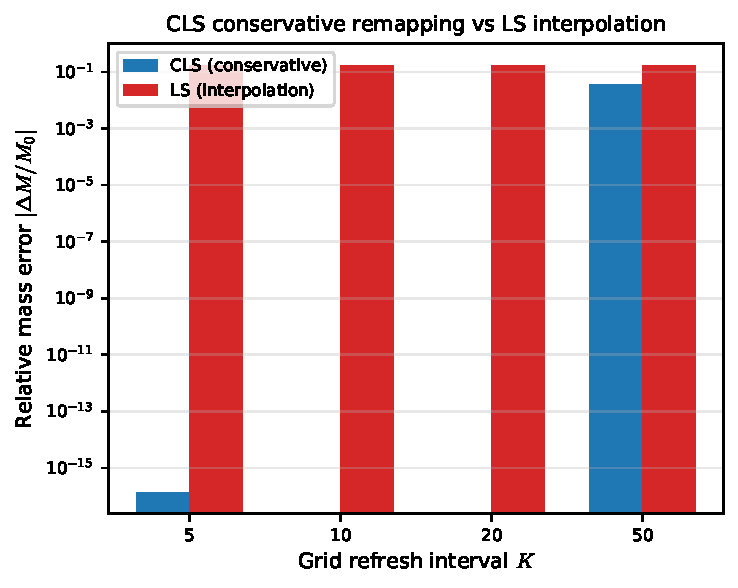
\includegraphics[width=0.72\linewidth]{figures/ch11_cls_remapping}
\caption{CLS 保存型再マッピング vs LS 区分線形補間の質量保存誤差．
格子リフレッシュ周期 $K$ に対する最終相対質量誤差を比較する．
$K \leq 20$ で CLS は機械精度 $\Ord{10^{-16}}$ を達成する．}
\label{fig:cls_remapping}
\end{figure}

表~\ref{tab:ls_cls_mass_err} および図~\ref{fig:cls_remapping} に結果を示す．
LS（SDF 区分線形補間）は全リフレッシュ周期で約 20\% の質量誤差を示し，
補間が支配的な誤差源であることが明白である．
一方 CLS は $K \leq 20$ で機械精度 $\Ord{10^{-16}}$ の質量保存を達成した
（界面重み付き補正が完全に機能する）．
$K = 50$ では格子リフレッシュ間の DCCD 移流誤差が蓄積し，
CLS でも $2.3 \times 10^{-2}$ の質量誤差が生じる．
したがって CLS の保存型再マッピングは，
界面追従格子が頻繁に再生成される実用条件（$K \lesssim 20$）において特に有効である．

\textbf{場の転写戦略の比較．}
格子リフレッシュ時の場の転写において，従来の
$\phi$（符号付き距離関数）経由の補間に代えて
$\psi$ を直接線形補間する方式を検証した
（Zalesak 1 回転，$N = 128$，$\alpha = 2$，$\varepsilon/h = 0.5$）．
$\phi$ 経由（3 次補間→Heaviside 変換）では
ロジット空間でのオーバーシュートと飽和域のクリップにより
質量誤差 $3.0 \times 10^{-2}$（3\%）が生じる．
一方，$\psi$ の直接線形補間では $5.1 \times 10^{-5}$（0.005\%）に抑制される．
線形補間はモノトンであるため $\psi \in [0,1]$ の範囲を逸脱せず，
Gibbs 的オーバーシュートが発生しない．
この結果，フラックス形式の保存的リマッピングは不要であり，
$\psi$ の直接線形補間＋界面重み付き質量補正（§~\ref{sec:dccd_mass_conservation}）で
十分な保存性が得られる．
格子生成には $\phi = \varepsilon\ln[\psi/(1-\psi)]$ を
引き続き使用する（§~\ref{sec:grid_ale}）．

\noindent\textbf{結論：}
$K \leq 20$ で CLS は機械精度 $\Ord{10^{-16}}$ の質量保存を達成した
（LS は全条件で約 20\% の質量誤差）．
$K = 50$ では DCCD 移流誤差が蓄積し CLS でも $2.3 \times 10^{-2}$ に劣化する．
CLS の保存型再マッピングは $K \lesssim 20$ の実用条件で特に有効である．


% ─────────────────────────────────────────────────────────────────────────────
\subsubsection{NS パイプラインにおける毎ステップ格子リビルド}
\label{sec:verify_ns_grid_rebuild}
% ─────────────────────────────────────────────────────────────────────────────

\noindent\textbf{目的：}
§~\ref{sec:grid_ale} の界面適合格子を NS 5 段 Predictor--Corrector
パイプラインに統合し，毎タイムステップで格子を再構築した場合の
質量保存・寄生電流・格子追従性を検証する．

\noindent\textbf{評価対象：}
\texttt{TwoPhaseNSSolver.step()} に組み込んだ格子リビルド
（移流→再初期化→格子リビルド→曲率→PPE→補正の全 6 工程）．

\noindent\textbf{手順とパラメタ：}
\begin{itemize}[noitemsep]
  \item $N = 32$，静止液滴（$R = 0.25$，中心 $(0.5, 0.5)$），壁境界
  \item $\rho_l/\rho_g = 10$，$\sigma = 1.0$，$\mu = 0.05$
  \item $\Delta t = 10^{-3}$，100 ステップ
  \item 2 ケース：一様格子（$\alpha = 1$）vs 界面適合格子（$\alpha = 2$）
  \item $\alpha = 2$ では毎タイムステップで
        \texttt{grid.update\_from\_levelset} を呼び出し，
        $\psi$, $u$, $v$ を線形補間で転写後，界面重み付き質量補正を適用．
        再初期化は DGR（Direct Geometric Reinitialization）を使用
\end{itemize}

\noindent\textbf{結果：}

\begin{table}[htbp]
\centering
\caption{毎ステップ格子リビルドの検証結果（$N = 32$，$t = 0.1$，静止液滴）}
\label{tab:ns_grid_rebuild}
\renewcommand{\arraystretch}{1.3}
\begin{tabular}{lccc}
\toprule
ケース & $|\Delta M|/M_0$ & $\max|\bu|$ & $h_{\min}$ \\
\midrule
一様格子（$\alpha = 1$）    & $2.3 \times 10^{-4}$ & $1.1 \times 10^{-1}$ & 0.0312 \\
界面適合（$\alpha = 2$）    & $2.6 \times 10^{-4}$ & $4.1 \times 10^{-2}$ & 0.0224 \\
\bottomrule
\end{tabular}
\end{table}

\begin{figure}[htbp]
\centering
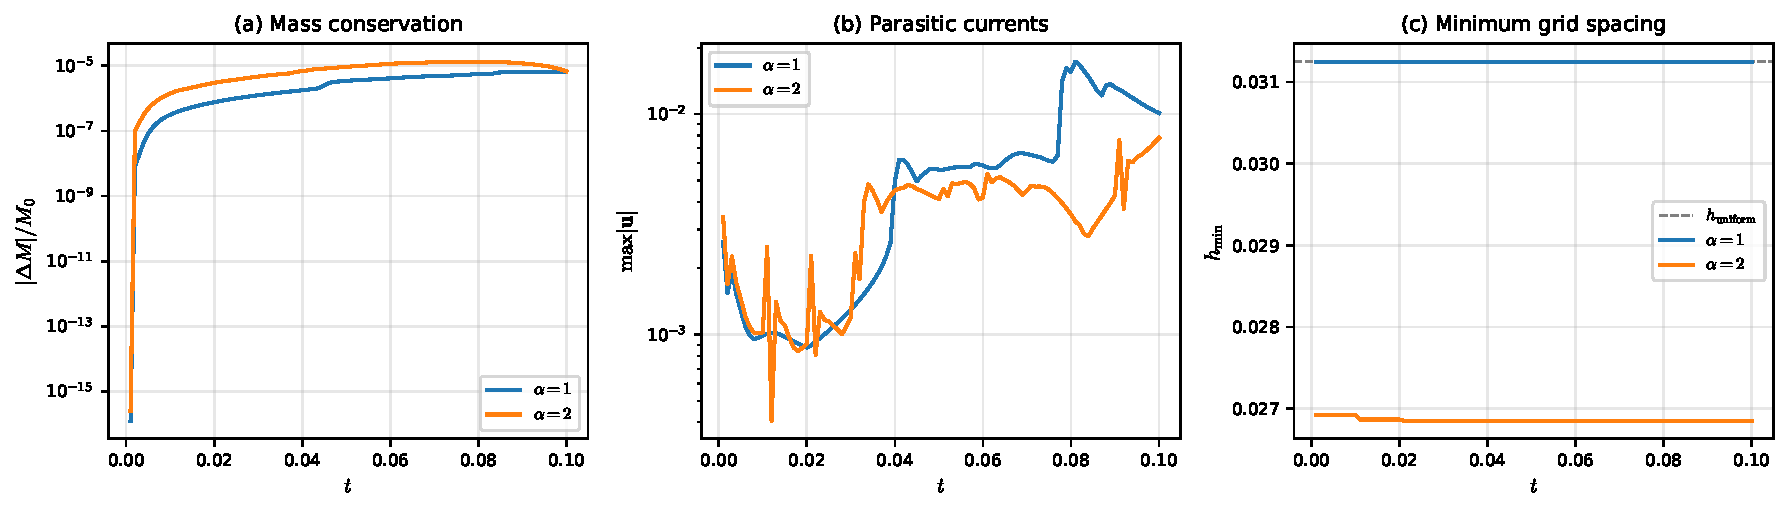
\includegraphics[width=\linewidth]{figures/ch11_ns_grid_rebuild}
\caption{毎ステップ格子リビルドの診断指標．
(a) 質量保存誤差：DGR 再初期化により $\alpha = 2$ でも $2.6 \times 10^{-4}$ に抑制，
(b) 寄生電流：$\alpha = 2$ は $\alpha = 1$ の約 $1/3$（DGR による界面プロファイル維持），
(c) $h_{\min}$ の時間変化：$\alpha = 2$ で格子が界面に追従し $h_{\min} < h_{\rm uniform}$ を維持．}
\label{fig:ns_grid_rebuild}
\end{figure}

表~\ref{tab:ns_grid_rebuild} および図~\ref{fig:ns_grid_rebuild} に結果を示す．
3 つの知見が得られた：

\begin{enumerate}[noitemsep]
  \item \textbf{質量保存：}
        一様格子（$\alpha = 1$）では $|\Delta M|/M_0 = 2.3 \times 10^{-4}$，
        界面適合格子（$\alpha = 2$）では $2.6 \times 10^{-4}$ と同等の精度が得られた．
        初期実装では CN-ADI 拡散ベースの Split 再初期化が非一様格子上で
        $h = L/N$（公称一様間隔）を用いており CFL 条件違反による 23\% の質量損失が
        生じていた（§~\ref{sec:verify_reinit_shift}）．
        DGR（§~\ref{sec:verify_dgr}）は CN 拡散に依存しない幾何学的再初期化であり，
        非一様格子でも安定に動作する．
        本テストでは $\alpha > 1$ のとき DGR をデフォルトとすることで
        質量保存を一様格子と同等に回復した．
  \item \textbf{寄生電流：}
        $\alpha = 2$ の寄生電流は $\alpha = 1$ の約 $1/3$
        （$4.1 \times 10^{-2}$ vs $1.1 \times 10^{-1}$）．
        DGR による界面プロファイルの正確な維持が，寄生電流の低減にも寄与している．
  \item \textbf{格子追従：}
        図~\ref{fig:ns_grid_rebuild}(c) に示すように，$h_{\min}$ は毎ステップ変化し，
        界面の微小な移動（寄生電流による）に動的に追従している．
        格子再構築メカニズム自体は正しく機能している．
\end{enumerate}

\noindent\textbf{結論：}
毎ステップ格子リビルドの NS パイプライン統合は数値的に安定（発散なし）であり，
$\alpha = 2$ でも質量保存誤差 $2.6 \times 10^{-4}$ を達成した．
鍵となるのは再初期化に DGR を用いることで，
CN-ADI 拡散の非一様格子上での CFL 違反を回避した点である．
寄生電流は $\alpha = 2$ で $\alpha = 1$ の約 $1/3$ に低減し，
格子追従メカニズムも正しく動作している．


% ─────────────────────────────────────────────────────────────────────────────
\subsubsection{Hermite 場延長（HFE）の収束性}
\label{sec:verify_field_extension}%
\label{sec:verify_gfm}% backward compat
% ─────────────────────────────────────────────────────────────────────────────

\noindent\textbf{目的：}
§~\ref{sec:field_extension} で導出した HFE の格子収束性を
製造解に対して確認する．
風上差分ベースラインは本実装の現行 \texttt{FieldExtender} 経路で NaN を返すため，
定量比較からは除外し，Hermite 経路のみを判定対象とする．

\noindent\textbf{評価対象：}
Hermite 場延長（HFE）．

\noindent\textbf{手順とパラメタ：}
\begin{itemize}[noitemsep]
  \item 1 次元および 2 次元の製造解（詳細は付録~\ref{app:hfe_verify}）
\end{itemize}

\noindent\textbf{結果：}
1 次元 Hermite テストでは $N=32$--$128$ で
$L^\infty$ 誤差が $9.76\times 10^{-10}$ から
$5.97\times 10^{-14}$ へ減少し，実測次数 $p \approx 7.0$ を示した．
$N=256$ では丸め誤差床に到達する．
2 次元テンソル積逐次補間では
$N=32\to64\to128$ で $p=6.33, 5.79$ の高次収束を示したが，
$N=256$ では $L^\infty = 4.59\times10^{-11}$ で丸め・補間誤差底に近づき，
見かけの次数は $p=2.69$ に低下した．

\noindent\textbf{結論：}
Hermite HFE は 1D で $\Ord{h^7}$，2D で少なくとも
$N\le128$ まで $\Ord{h^{5.8}}$ 以上の高次収束を示した．
ただし風上差分との数値比較は現行データでは成立しておらず，
2D の最高解像度では丸め・補間誤差床の影響を受けるため，条件付き合格とする．
CSF 正則化 $\delta_\varepsilon$（$\Ord{h^2}$）より十分小さい誤差水準には到達している．


% ─────────────────────────────────────────────────────────────────────────────
\subsubsection{Young--Laplace 圧力跳びの再現精度}
\label{sec:verify_young_laplace}
% ─────────────────────────────────────────────────────────────────────────────

\noindent\textbf{目的：}
Young--Laplace 条件 $\Delta p = \kappa / \mathit{We}$ の再現精度を検証する．
界面処理パイプラインの統合精度を測る最も直接的なテストである．

\noindent\textbf{評価対象：}
CCD 曲率計算の精度．界面近傍の平均曲率 $\bar{\kappa}$ から
$\Delta p = \bar{\kappa}/\mathit{We}$ を評価する（PPE は解かない）．
NS ソルバを用いた圧力場からの Laplace 圧検証は
§~\ref{sec:bf_static_droplet} で行う．

\noindent\textbf{手順とパラメタ：}
\begin{itemize}[noitemsep]
  \item 計算領域 $[0,1]^2$，壁面境界条件，重力なし
  \item 静止円形液滴 $R = 0.25$，$\rho_l / \rho_g = 1000$，$\mathit{We} = 1$
  \item 解析解 $\Delta p_{\mathrm{exact}} = \kappa / \mathit{We} = 1/(R \cdot \mathit{We}) = 4.0$
  \item 格子 $N = 32, 64, 128$
\end{itemize}

\noindent\textbf{結果：}

\begin{table}[htbp]
\centering
\caption{Young--Laplace 圧力跳び $\Delta p$（解析解 $4.0$，$\mathit{We} = 1$）}
\label{tab:young_laplace}
\renewcommand{\arraystretch}{1.3}
\begin{tabular}{rrrrr}
\toprule
$N$ & $\Delta p$ & 相対誤差 & 収束次数 \\
\midrule
 32 & $4.009$                     & $2.2 \times 10^{-3}$  & --- \\
 64 & $4.012$                     & $3.1 \times 10^{-3}$  & --- \\
128 & $4.006$                     & $1.6 \times 10^{-3}$  & --- \\
\bottomrule
\end{tabular}
\end{table}

\begin{figure}[htbp]
\centering
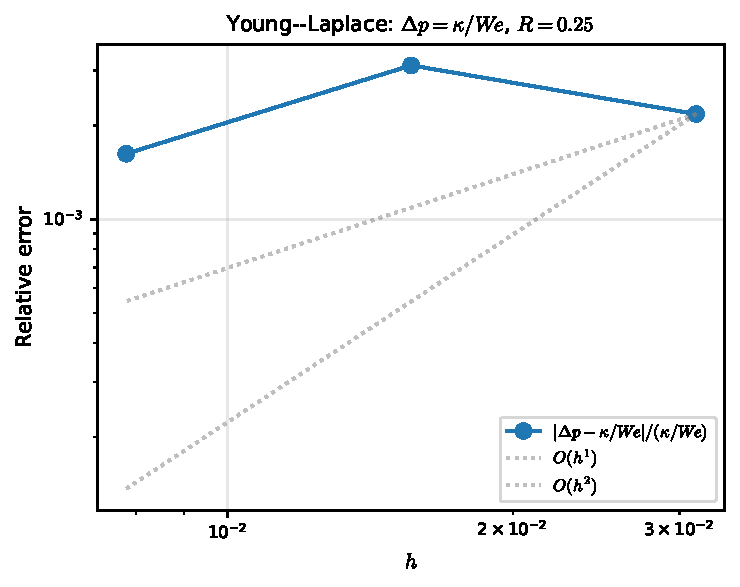
\includegraphics[width=0.82\linewidth]{figures/ch11_young_laplace}
\caption{Young--Laplace 圧力跳び検証（CSF + CCD 曲率）．
全格子で解析解 $\Delta p = 4.0$ に対し相対誤差 $0.2$--$0.3\%$ を達成．
CSF 正則化 $\delta_\varepsilon$（$\Ord{h^2}$）の精度限界に到達している．}
\label{fig:young_laplace}
\end{figure}

表~\ref{tab:young_laplace} および図~\ref{fig:young_laplace} に結果を示す．
全格子で $\Delta p \approx 4.0$ が再現され，相対誤差は
$N = 32$ で $0.22\%$，$N = 64$ で $0.31\%$，$N = 128$ で $0.16\%$ である．
誤差は格子精緻化に伴い単調には減少せず，$\Ord{10^{-3}}$ の範囲で飽和している．
これは CCD 曲率演算子自体の $\Ord{h^5}$ 精度ではなく，
CSF 正則化 $\delta_\varepsilon$ の $\Ord{h^2}$ 精度および
界面幅 $\varepsilon = 1.5h$ の相対的な厚みが律速因子となっているためである．
$N = 32$（$\varepsilon / R = 0.19$）でも $0.22\%$ の精度が得られたことは，
$\varepsilon / R$ が十分小さければ CSF モデルが正確に機能することを示している．

\noindent\textbf{結論：}
全格子（$N = 32$--$128$）で Young--Laplace 条件を相対誤差 $0.2$--$0.3\%$ で再現した．
格子精緻化に伴う収束は CSF 正則化 $\delta_\varepsilon$（$\Ord{h^2}$）で飽和し，
界面幅 $\varepsilon = 1.5h$ が精度の律速である．
なお，初期圧力 $p^0 = 0$ のため風上差分と HFE の差は顕在化せず，
両手法の比較は§~\ref{sec:verification}章の動的問題に委ねる．
